%*******************************************************************************
%*********************************** Third Chapter *****************************
%*******************************************************************************

\chapter{Study Frameworks}  %Title of the Third Chapter
\section{Theoretical Framework}

The theoretical framework illustrates the different theories involved in this study and how they relate to each other in order to achieve the study's objective. Figure 3.1 below shows this study's theoretical framework.
\begin{figure}[H]
    \centering
    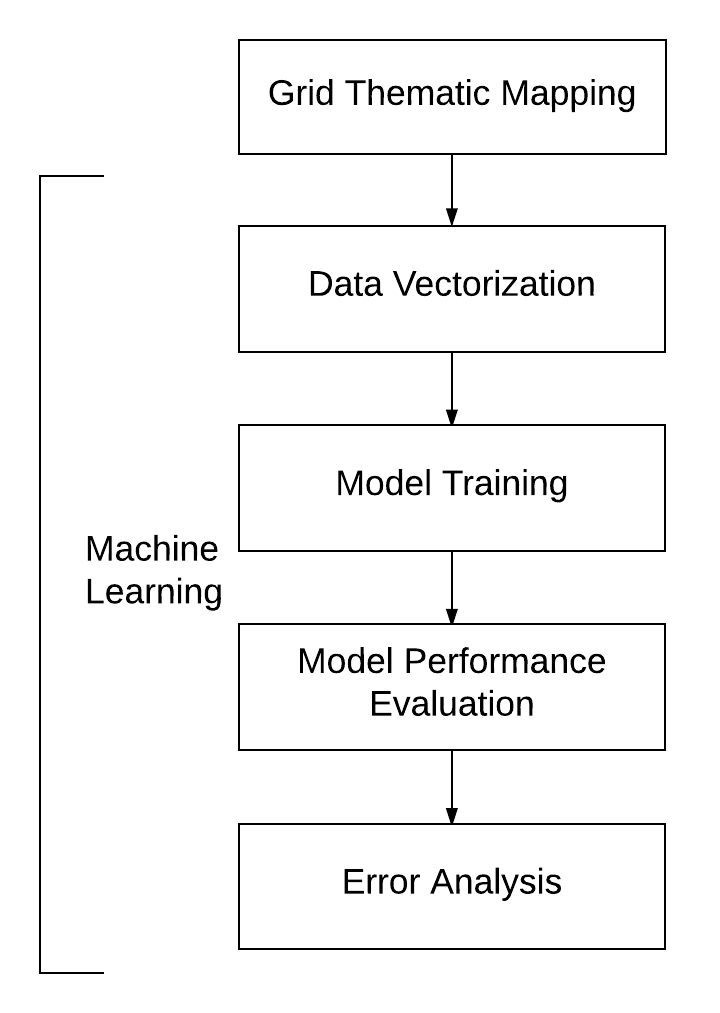
\includegraphics[width=7cm]{theoretical-framework}
    \caption{The theoretical framework of the study}
\end{figure}
In order to map crimes, we need a way to generate hotspots \citep{eck2005mapping}. By generating possible hotspots, we can easily analyze crimes and map them. One of the easiest and fastest way to identify hotspots is grid thematic mapping \citep{chainey2008utility}. Grid thematic mapping is done through placing uniform cells over a geographical area and thematically shading them. Problems involving different shapes and dimensions of geographical areas can be addressed and dealing with consistent dimensions allows easier and quicker analysis and comparison.

After generating the grid, we can commence machine learning. Machine learning is the study and computer modeling of learning processes and algorithms \citep{michalski2013machine}. In the case of this study, crime hotspots will be learned and predicted through a model employing the algorithm of Recurrent Neural Network (RNN) with Long Short-term Memory (LSTM) architecture. 

Machine learning starts by generating our data vectors. Meaningful data is extracted from the information expressed by the presence and absence of criminal records in the different cells generated through grid thematic mapping.

The LSTM model is then trained with this data in order to learn the nature of crime with respect to the cells in the grid. The LSTM network learns by storing data representation of previous input events in forms of activation embodied by the weighted connections between gates and inputs/outputs \citep{hochreiter1997long}. It processes data using the following set of functions as described by Graves \citeyearpar{graves2013generating} and as illustrated and explained in Section 2.6 of this paper. The output \( h_t \) of the LSTM layer at timestep $t$ is the function of the input for the input \( x_t \) and the output \( h_{t-1} \) and cell state \( C_{t-1} \) of the layer from the previous timestep by:
    \begin{align}
    i_t &= \sigma(x_t W_{xi} + h_{t-1} W_{hi} + C_{t-1} W_{Ci} + b_i) \\
    f_t &= \sigma(x_t W_{xf} + h_{t-1} W_{hf} + C_{t-1} W_{Cf} + b_f) \\
    C_t &= f_t C_{t-1} + i_t \tanh(x_t W_{xC} + h_{t-1} W_{hC} + b_C) \\
    o_t &= \sigma(x_t W_{xo} + h_{t-1} W_{ho} + C_t W_{Co} + b_o) \\
    h_t &= o_t \tanh(C_t)
    \end{align}

The three gates of an LSTM, namely the input \( i_t \), forget \( f_t \) and output \( o_t \) gates are activated for the current timestep $t$ using the equations (3.1), (3.2) and (3.4) respectively. The cell state for the layer \( C_t \) is updated using equation (3.3). Finally, the output for the current layer \( h_t \) is produced by equation (3.5). The value \(W_{ab}\) is the weighted connection between $a$ and $b$ so \(W_{xC}\), for instance, denotes the weighted connection between the input node of the current layer and the cell state. The LSTM network goes through all the inputs and outputs and adjusts its weight matrix, or the different values of $W$, accordingly. The final model will have a set of weight matrix that is applied to future inputs to predict outputs.

After training, the LSTM model must undergo tests and experiments as part of machine learning in order to assess its performance. It is important to measure the accuracy and precision of the model in order to evaluate if it performed well or not. To understand why it performed as such, error analysis is also done.